\documentclass[hidelinks,11pt,dvipsnames]{article}
% xcolor commonly causes option clashes, this fixes that
\PassOptionsToPackage{dvipsnames,table}{xcolor}
\usepackage[tmargin=1in, bmargin=1in, lmargin=0.8in, rmargin=1in]{geometry}

%%%%%%%%%%%%%%%%%%%%%%%%%%%%%%%%%%%%%%%%%%%%%%%%%%%%%%%%%%%%%%%%%%%%
%%% For inkscape-figures
%%% Assumes the following directory structure:
%%% master.tex
%%% figures/
%%%     figure1.pdf_tex
%%%     figure1.svg
%%%     figure1.pdf
%%%%%%%%%%%%%%%%%%%%%%%%%%%%%%%%%%%%%%%%%%%%%%%%%%%%%%%%%%%%%%%%%%%%
%\usepackage{import}
\usepackage{pdfpages}
\usepackage{transparent}

\newcommand{\incfig}[2][1]{%
    \def\svgwidth{#1\columnwidth}
    \import{./figures/}{#2.pdf_tex}
}

\pdfsuppresswarningpagegroup=1

% enable synctex for inverse search, whatever synctex is
\synctex=1
\usepackage{float,macrosabound,homework,theorem-env}
\usepackage{microtype}


% font stuff
\usepackage{sectsty}
\allsectionsfont{\sffamily}
\linespread{1.1}

% bibtex stuff
\usepackage[backend=biber,style=alphabetic,sorting=anyt]{biblatex}
\addbibresource{main.bib}

% colored text shortcuts
\newcommand{\blue}[1]{\color{MidnightBlue}{#1}}
\newcommand{\red}[1]{\textcolor{Mahogany}{#1}}
\newcommand{\green}[1]{\textcolor{ForestGreen}{#1}}


% use mathptmx pkg while using default mathcal font
\DeclareMathAlphabet{\mathcal}{OMS}{cmsy}{m}{n}

% fixes the positioning of subscripts in $$ $$
\renewcommand{\det}{\operatorname{det}}

\usetikzlibrary{positioning, arrows.meta}
\newcommand{\here}[2]{\tikz[remember picture]{\node[inner sep=0](#2){#1}}}

%%%%%%%%%%%%%%%%%%%%%%%%%%%%%%%%%%%%%%%%%%%%%%%%%%%%%%%%%%%%%%%%%%%%%
%%% Entry Counter
%%%%%%%%%%%%%%%%%%%%%%%%%%%%%%%%%%%%%%%%%%%%%%%%%%%%%%%%%%%%%%%%%%%%%
\newcounter{entry-counter}
\newcommand{\entry}[1]
{
	\addtocounter{entry-counter}{1}
    \tchap{Entry \arabic{entry-counter}}
	%\addcontentsline{toc}{section}{Entry \arabic{entry-counter}: #1}
	\vspace{-1.5em}
    \begin{center}
		\small \emph{Written: #1}
    \end{center}
}

\usepackage{titling}
\renewcommand\maketitlehooka{\null\mbox{}\vfill}
\renewcommand\maketitlehookd{\vfill\null}


\usepackage{capt-of}
\usepackage{tikz}
\usetikzlibrary{positioning,calc,intersections,through,backgrounds, shapes.geometric, decorations.markings,arrows}

\def\sset{\subseteq}
\def\iso{\cong}
\def\gend#1{\langle #1\rangle}

\newcommand{\rightoverleftarrow}{%
  \mathrel{\vcenter{\mathsurround0pt
    \ialign{##\crcr
      \noalign{\nointerlineskip}$\longrightarrow$\crcr
      \noalign{\nointerlineskip}$\longleftarrow$\crcr
    }%
  }}%
}

\newcommand\makesphere{} % just for safety
\def\makesphere(#1)(#2)[#3][#4]{%
  % Synopsis
  % \makesphere[draw options](center)(initial angle:final angle:radius)
  \shade[ball color = #3, opacity = #4] #1 circle (#2);
  \draw #1 circle (#2);
  \draw ($#1 - (#2, 0)$) arc (180:360:#2 and 3*#2/10);
  \draw[dashed] ($#1 + (#2, 0)$) arc (0:180:#2 and 3*#2/10);
}
% same thing as makesphere but places white background behind
\newcommand\altmakesphere{} % just for safety
\def\altmakesphere(#1)(#2)(#3)[#4][#5]{%
  % Synopsis
  % \make sphere[draw options](center)(initial angle:final angle:radius)
  \draw [fill=white!30] #1 circle (#2);
  \shade[ball color = #4, opacity = #5] #1 circle (#2);
  \draw #1 circle (#2);
  \draw ($#1 - (#2, 0)$) arc (180:360:#2 and 3*#2/10);
  \draw[dashed] ($#1 + (#2, 0)$) arc (0:180:#2 and 3*#2/10);
  \node at #1 {#3};
}

\begin{document}
\pagestyle{empty}
	\LARGE
\begin{center}
	Algebraic Topology Homework 7 \\
	\Large
	Isaac Martin \\
    Last compiled \today
\end{center}
\normalsize
\vspace{-4mm}
\hru

\tchap{Problems from 2.1}

\begin{homework}[e]
  \prob[2.1.1] What familiar space is the quotient $\Delta$-complex of a 2-simplex $[v_0, v_1,v_2]$ obtained by identifying the edges $[v_0,v_1]$ and $[v_1,v_2]$ preserving the ordering of vertices?
  \begin{prf}
    The space we obtain is a copy of the M\"obius band. This is more obvious if we perform some cuts and pastes (thank you for the suggestion Jacob): 
    \begin{center}
      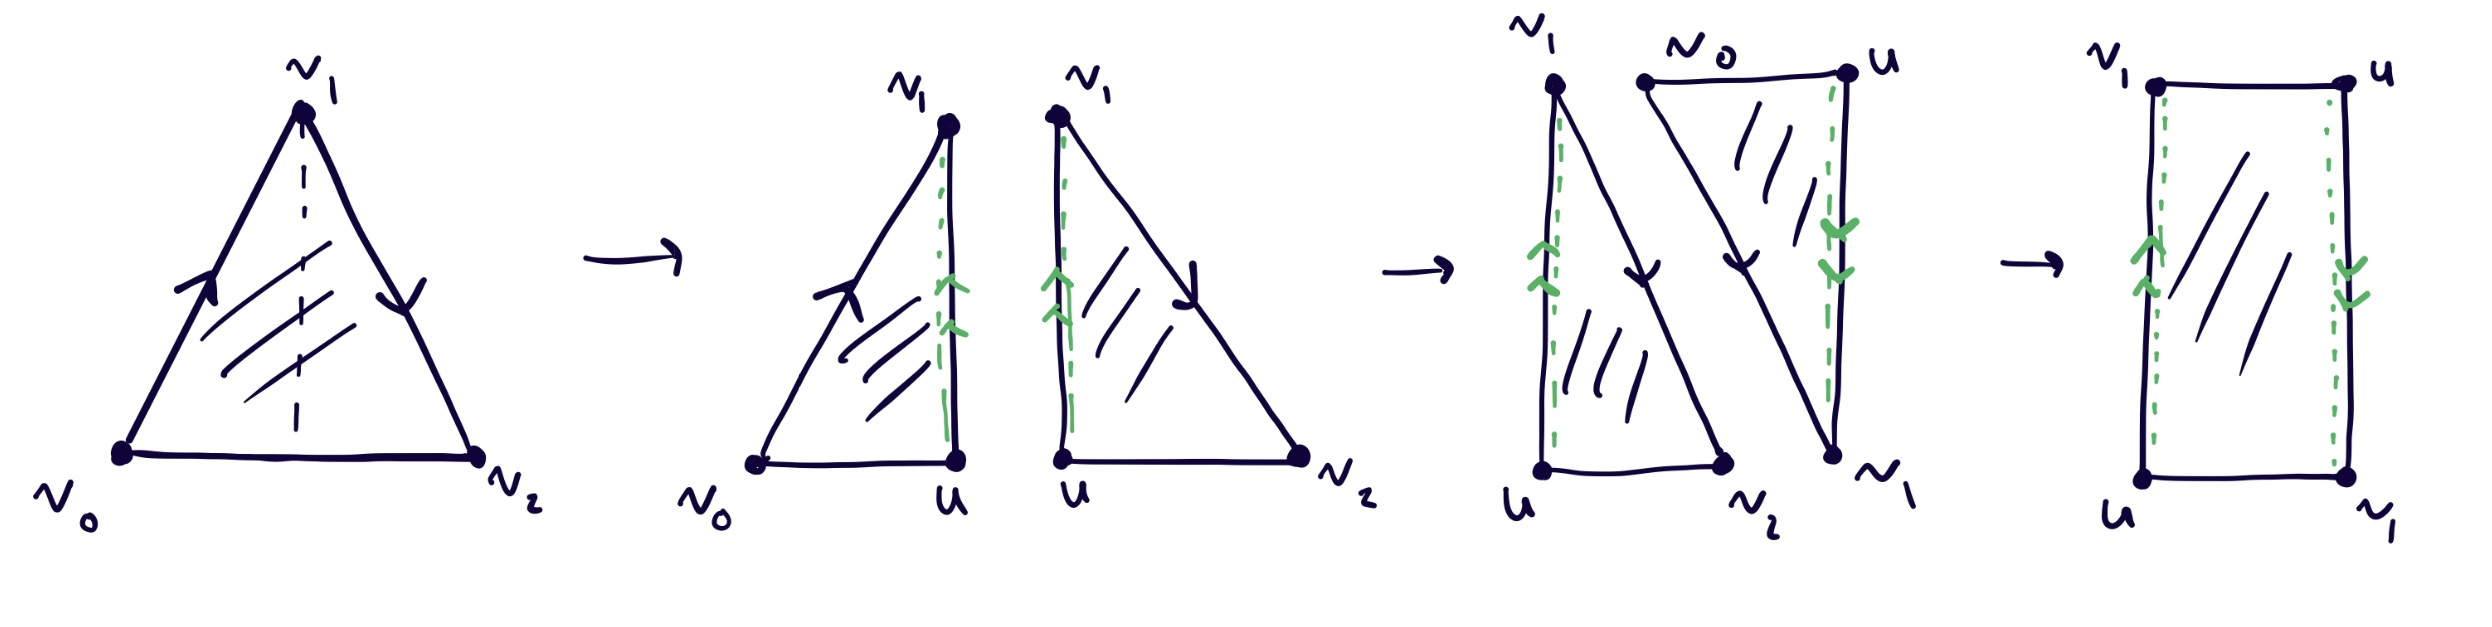
\includegraphics[width=14cm]{figures/hwk7-fig4.png}
      \captionof{figure}{Cut and gluing operation making it clear we obtain a M\"obius band} 
      \label{fig:prob2-4}
    \end{center}
    I initially thought the given identification produced a ``hollow cone'', but this is not the case since it preserves orientation of the edges. Were we to reverse the orientation of one of the edges involved in the identification, i.e. identify $[v_0,v_1]$ with $[v_2,v_1]$, then we would indeed obtain a cone.
  \end{prf}
  \prob[2.1.2] Show that the $\Delta$-complex obtained from $\Delta^3$ by performing the order-preserving edge identifications $[v_0,v_1]\sim [v_1,v_3]$ and $[v_0,v_2]\sim [v_2,v_3]$ deformation retracts onto a Klein bottle. Also, find other pairs of identifications of edges that produce $\Delta$-complexes deformation retracting onto a torus, a $2$-sphere, and $\bRP^2$.
  \begin{prf}
    The deformation retraction takes the tetrahedron $\Delta^3$ to a square with edges $[v_0,v_1]$, $[v_1,v_3]$, $[v_0,v_2]$ and $[v_2,v_3]$. 
    \begin{center}
      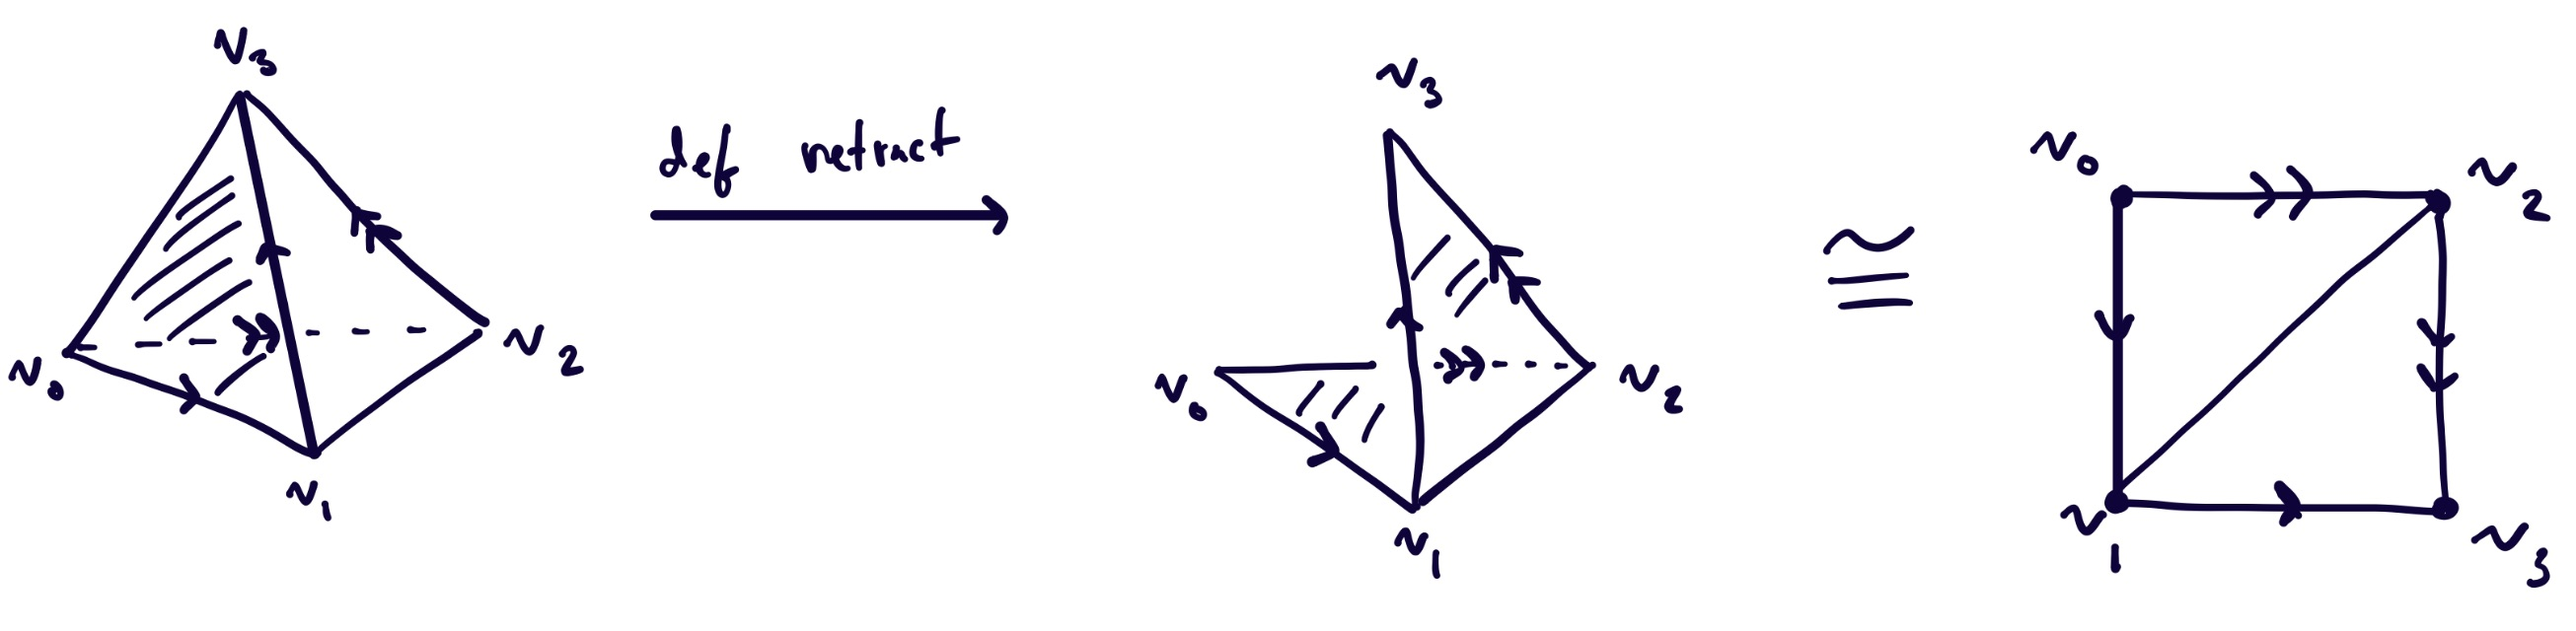
\includegraphics[width=14cm]{figures/hwk7-fig1.png}
      \captionof{figure}{Deformation retract of $\Delta^3$ onto a square} 
      \label{fig:prob2-1}
    \end{center}
    From here, cutting along the diagonal $[v_1,v_2]$, rearranging the resulting copies of $\Delta^2$ and gluing back together yields the standard polygon of the Klein bottle. 
    \begin{center}
      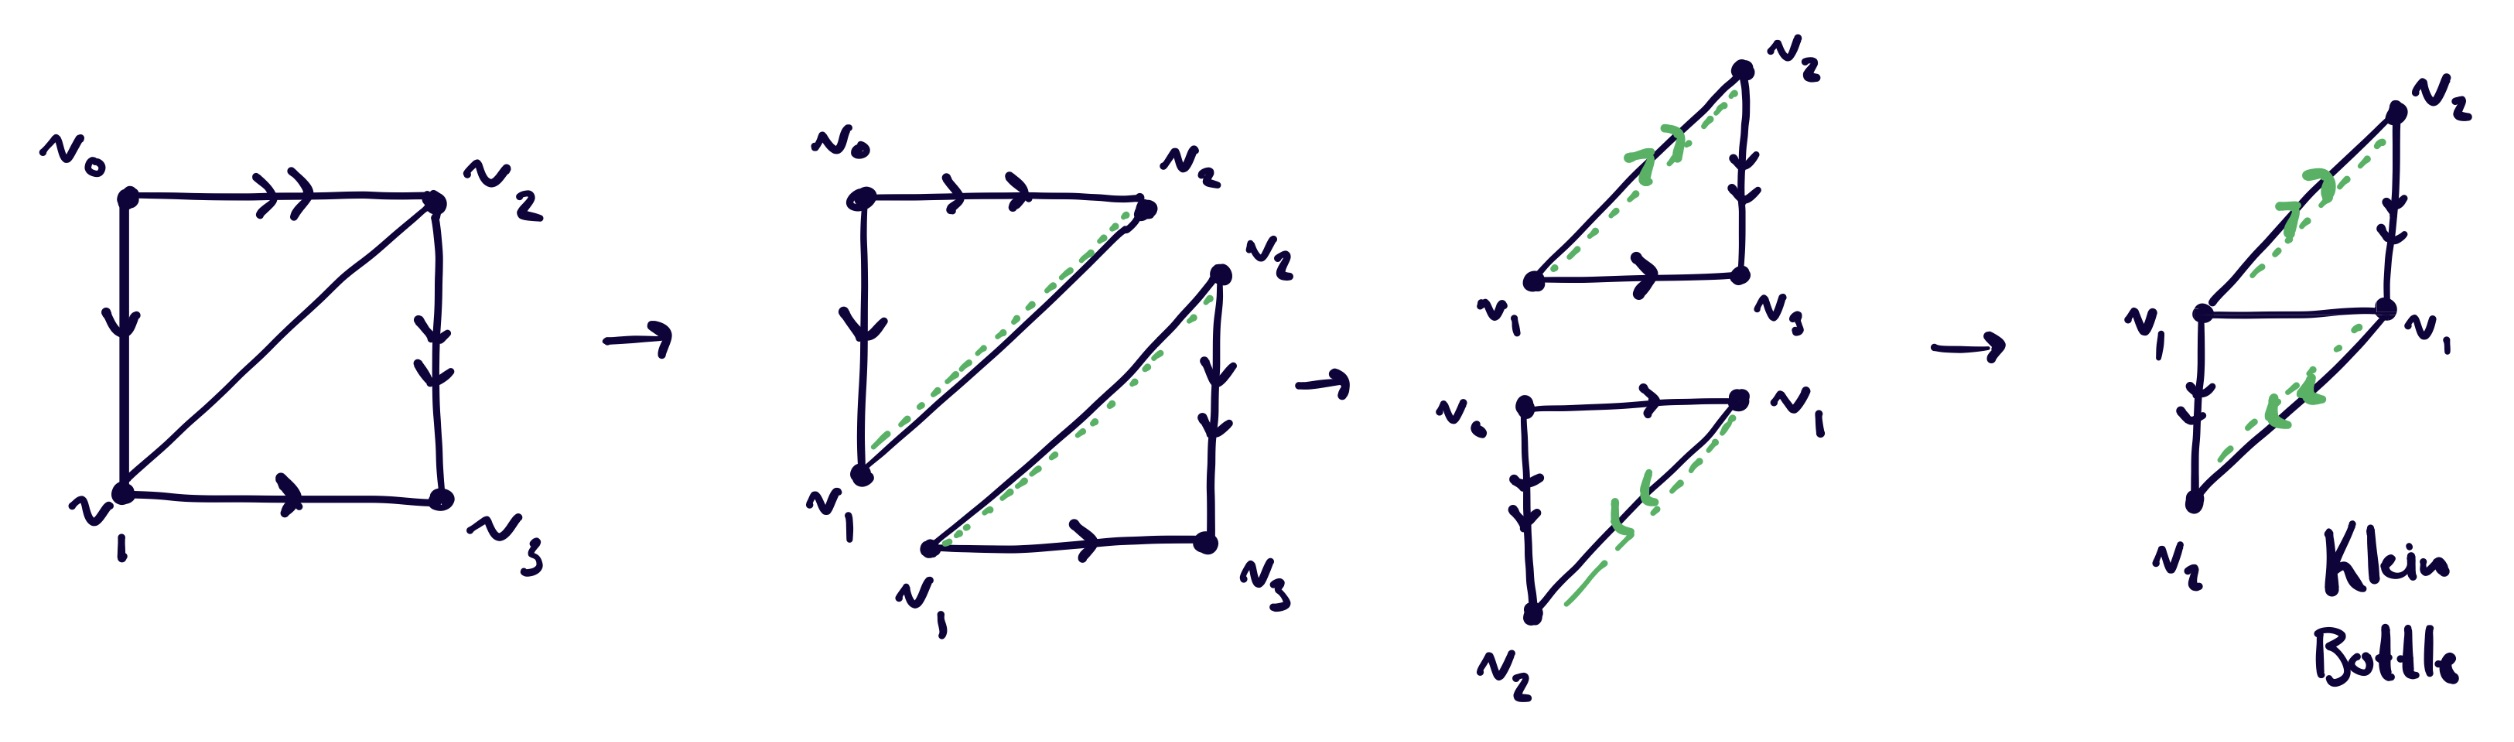
\includegraphics[width=14cm]{figures/hwk7-fig2.png}
      \captionof{figure}{Rearrangement of square to obtain fundamental polygon of the Klein bottle} 
      \label{fig:prob2-2}
    \end{center}

    Here we list the identifications needed to construct the torus, the 2-dimensional sphere and $\bRP^2$. I drew these on the chalkboard but did not replicate them for the submission -- as this process is nearly identical to what we did for the Klein bottle, I hope the lack of a picture is permissible.
    \begin{enumerate}[(i)]
      \item $T^2:$ $[v_0,v_1] \sim [v_1,v_3]$ and $[v_0,v_1]\sim [v_2,v_3]$
      \item $S^2$: $[v_0,v_2]\sim [v_3,v_2]$ and $[v_0,v_2]\sim [v_3,v_1]$
      \item $\bRP^2$: $[v_0,v_2]\sim [v_3,v_1]$ and $[v_0,v_1]\sim [v_3,v_2]$
    \end{enumerate}
    Note that these identifications don't necessarily preserve the orientation of vertices.
  \end{prf}

  \prob[2.1.3] Construct a $\Delta$-complex structure on $\bRP^n$ as a quotient of a $\Delta$-complex structure on $S^n$ having vertices the two vectors of length $1$ along each coordinate axis in $\bR^{n+1}$.
  \begin{prf}
    Here we simply construct the space specified in Hatcher to obtain a space homeomorphic to $S^n$ and then mod out by $x \sim -x$ to obtain $\bRP^n$. The construction goes as follows.
    
    Let $e_i^+ \in \bR^{n+1}$ denote the standard $i$th orthonormal basis vector for $\bR^{n+1}$, and let $e_i^- = -e_i^{+}\in \bR^{n+1}$ denote the corresponding basis vector with $-1$ in the $i$th position rather than $1$. Consider then the collection of $n$-cells of the form $[v_1,...,v_{n+1}]$ (of which there are $2^{n+1}$) where $v_i \in \{e_i^+,e_i^-\}$ and glue these along shared $n-1$ simplicies. For example, in $\bR^2$, we glue $[e_1^+,e_2^+,e_3^+]$ and $[e_1^+,e_2^+,e_3^-]$ along their shared 1-simplex $[e_1^+,e_2^+]$. Neither one of these $2$-simplicies is glued to $[e_1^-,e_2^-,e_3^+]$ however, as neither shares an edge with it. The resulting $\Delta$-complex (returning to the arbitrary $n$ case) is then homeomorphic to $S^n$, and once we quotient by the relation $x \sim -x$ we obtain $\bRP^n$. In terms of simplicies, we identify $[v_1,...,v_{n+1}]$ with $[-v_1,...,-v_{n+1}]$ where again $v_i \in \{e_i^+,e_i^-\}$.
    \begin{center}
      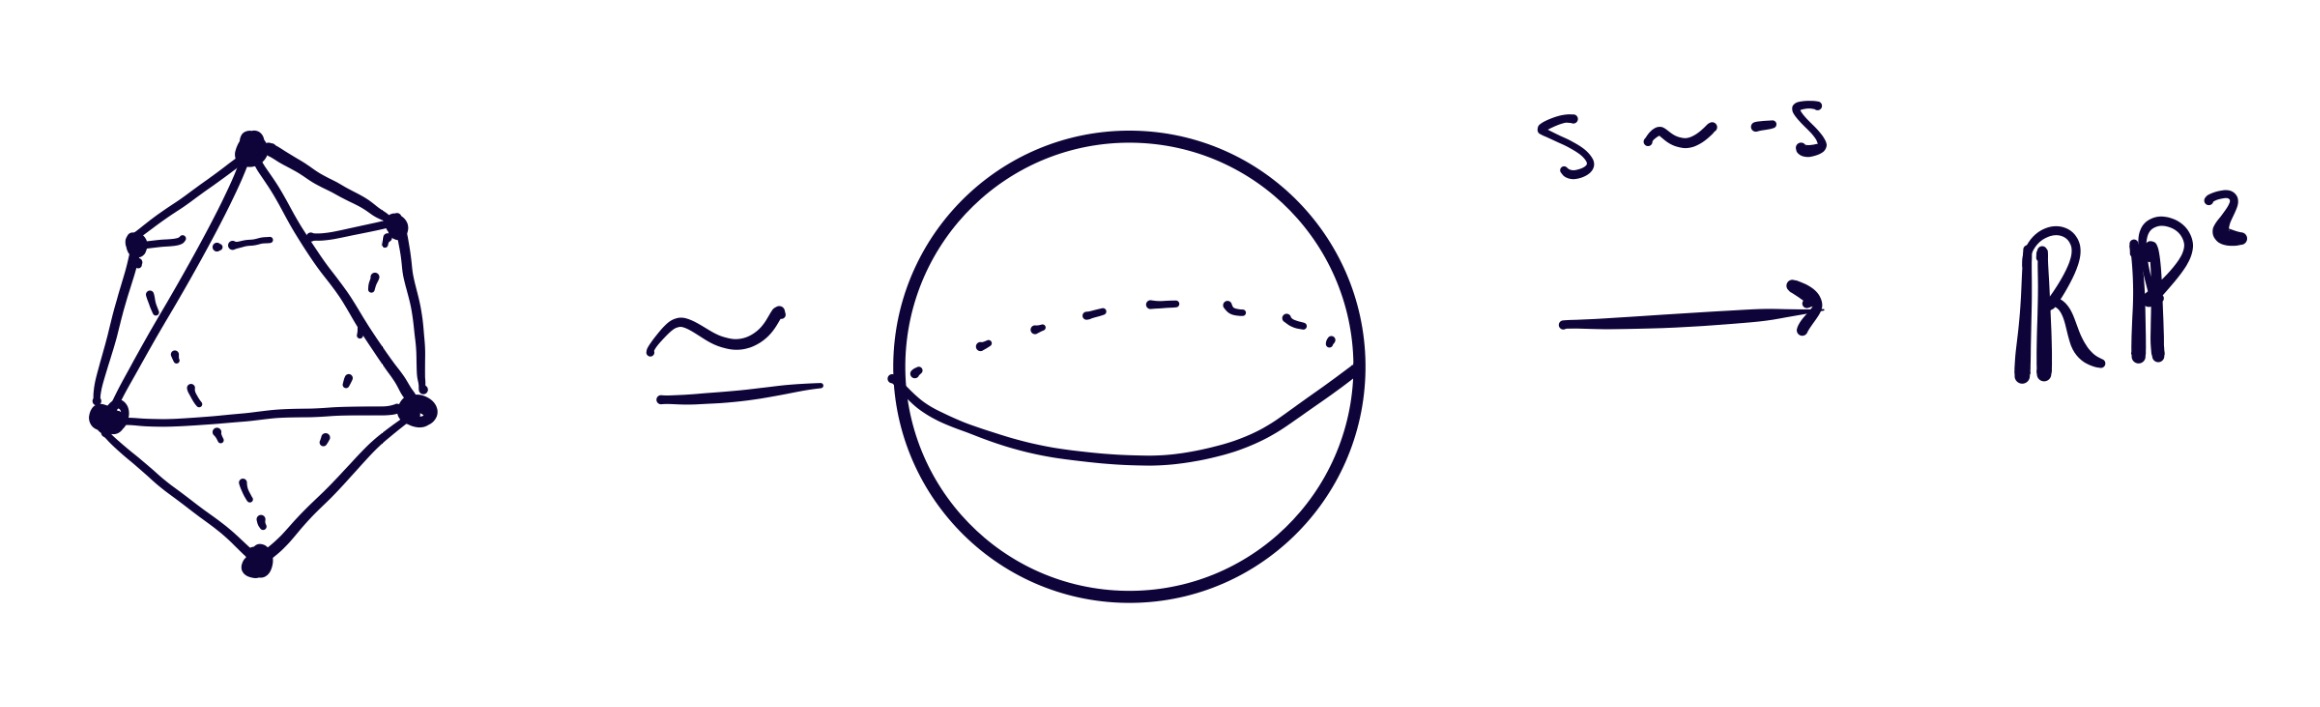
\includegraphics[width=12cm]{figures/hwk7-fig3.png}
      \captionof{figure}{Obtaining $\bRP^2$ as a quotient of a $\Delta$-complex structure on $S^2$}
      \label{fig:prob2-3}
    \end{center}
  \end{prf}
  \prob[2.1.14] Determine whether there exists a short exact sequence $0 \to \bZ_4 \to \bZ_8 \oplus \bZ_2 \to \bZ_4 \to 0$. More generally, determine which abelian groups $A$ fit into a short exact sequence $0 \to \bZ_{p^m} \to A\to \bZ_{p^n}\to 0$ with $p$ prime. What about the case of short exact sequences $0 \to \bZ\to A\to \bZ_n \to 0$?
  \begin{prf}
    We break this into parts.

    (a) ~ Let's first define a map $\alpha:\bZ_4 \to \bZ_8\oplus \bZ_2$. This map is fully determined by the image of $1$ since $\bZ_4$ is cyclic, and in order for our sequence to be exact, $\alpha$ must be injective and hence the generator of $\bZ_4$ must be sent to an element of order $4$. If $\alpha(1)$ were less than order $4$ then the map wouldn't be injective, and if $\alpha(1)$ had order larger than $4$ then $\alpha(4) = 4\alpha(1)$ wouldn't be zero. Define $\alpha(1) = (2,1)$, which is indeed an element of order 4 in $\bZ_8\oplus \bZ_2$. This means $\img(\alpha) = \{(2,1),(4,0),(6,1),(0,0)\}$.

    I claim we can find a map $\beta:\bZ_8\oplus \bZ_2 \to \bZ_4$ which makes this sequence exact. Indeed, defining $\beta((1,0)) = 1$ and $\beta((0,1)) = 0$ fully determines a homomorphism $\bZ_8\oplus \bZ_2$ since $(1,0)$ and $(0,1)$ generate $\bZ_8\oplus \bZ_2$ and $\ker(\beta) = \{(2,1), (4,0),(6,1),(0,0)\} = \img(\alpha)$. Since we additionally have that $\alpha$ is injective and $\img(\beta) = \bZ_4$, as one can exhaustively check, the sequence
    \begin{align*}
      0 \to \bZ_4 \xrightarrow{\alpha} \bZ_8 \oplus \bZ_2 \xrightarrow{\beta} \bZ_4 \to 0
    \end{align*}
    is short exact.

    For fun, note that if we instead defined $\alpha(1) = (2,0)$, then the image of $\alpha$ would become $\{(2,0),(4,0),(6,0),(0,0)\}$. In this case, $(\bZ_8 \oplus \bZ_2)/\img(\alpha) \cong \bZ_2 \oplus \bZ_2 \not\cong \bZ_4$, so the choice of $\alpha(1)$ does indeed matter.

    \bigskip

    (b) ~ Now consider $0 \to \bZ_{p^m}\xrightarrow{\alpha} A \xrightarrow{\beta}\bZ_{p^n}\to 0$. We wish to find all such abelian groups $A$ for which there exist $\alpha$ and $\beta$ making this sequence exact. We immediately note that such an $A$ must satisfy $\bZ_{p^n}\cong A/\bZ_{p^m}$, with $\bZ_{p^m}$ identified with its image in $A$ under the injective map $\alpha$, and hence $|A| = p^np^m = p^{n+m}$. (Note that throughout (b) and (c) we will use the natural $\bZ$-action on abelian groups without comment. This is nice since it allows us to write things like $\alpha(k) = k\alpha(1)$ without worrying whether $k$ belongs to $A$ or $\bZ_{p^m}$.)

    Since $A$ is a finite Abelian group, by the structure theorem for finite abelian groups (or the fundamental theorem of abelian groups, whichever name you prefer) $A$ must have a decomposition
    \begin{align*}
      A \cong \bZ_{p^{k_1}} \oplus ... \oplus \bZ_{p^{k_\ell}}
    \end{align*}
    where $k_1 + ... + k_\ell = n+m$ and $k_i \geq 0$ for all $1\leq i\leq \ell$. We need only determine viable $\ell$ and $k_i$.

    Let's first find $\ell$. Consider an element $x \in A$ and set $a = \alpha(1)$ and $b \in A$ to be the element such that $\beta(b) = 1 \in \bZ_{p^n}$, which necessarily exists if $\beta$ is surjective. If $x\not\in \img(\alpha)$, then $\beta(x) \neq 0$ because $\img(\alpha) = \ker(\beta)$. There must then exist some $0\neq s \in \bZ_{p^n}$ such that $\beta(x) = s$. We then have that $\beta(x) = s\beta(b) = \beta(sb)$ since $\beta$ is a homomorphism, and furthermore that $\beta(x - sb) = 0\implies x - sb \in \ker(\beta)$. Again, because $\ker(\beta) = \img(\alpha)$, $x - sb \in \img(\alpha)$ and hence there is some $t \in \bZ_{p^m}$ such that
    \begin{align*}
      ta = t\alpha(a) = \alpha(ta) = x - sb \implies x = ta + sb.
    \end{align*}
    This shows that $x$ is in the subgroup of $A$ generated by $a$ and $b$, and since $x$ was chosen arbitrarily that $A$ is generated by two elements, so $\ell \leq 2$

    If $ra = b$ for some $r \in \bZ$, then $b = ra\in \img(\alpha) = \ker(\beta)$ and hence $\beta(b) = 0 = 1$. In this case, both $n = m = 0$ and both $\bZ_{p^n}$ and $\bZ_{p^m}$ are the trivial group, implying that $A$ is also the trivial group. If $b$ is not in the subgroup generated by $a$, then $A$ is generated by two independent elements and hence
    \begin{align*}
      A \cong \bZ_{p^{m+n-c}} \oplus \bZ_{p^c}
    \end{align*}
    for some $0\leq c\leq m+n$. However, since $\bZ_{p^m}$ injects into $A$, $A$ necessarily contains an element of order $p^m$. This occurs if and only if $m \leq \max\{m + n - c, c\}$ or equivalently $0\leq c \leq \min\{m,n\}$.

    Now define $\alpha$ by $\alpha(1) = (p^{n-c},1)$. Actually, since the definition of $\alpha$ now depends on $c$, denote it by $\alpha_c$. Because our sequence is exact if and only if $\bZ_{p^n} \cong A/\alpha_c(\bZ_{p^m})$ and $\bZ_{p^n}$ is cyclic, we need only show that there is some coset $x + \alpha_c(\bZ_{p^{m}})$ of order $p^n$. Set $H = \alpha_c(\bZ_{p^n})$ and suppose we have some arbitrary coset $(x,y) + H$. Then $(x,y) - y(p^{n-c},1)$ represents the same coset as $(x,y)$ because their difference is in $H$. However,
    \begin{align*}
      (x,y) - y(p^{n-c},1) = (x - yp^{n-c},0) = (x - yp^{n - c})\cdot (1,0),
    \end{align*}
    meaning that $(x,y) - y(p^{n-c},1) + H$ and hence $(x,y) + H$ is represented by a multiple of $(1,0)$. In particular, each $0\leq c \leq n - 1$ yields a unique coset so that $(1,0) + H = $ has order $p^n$. Hence $(1,0) + H$ generates the quotient $A/H$ since the quotient has order $p^n$. This implies that $\bZ_{p^m} \cong A/H$, and hence we may take $\beta_t$ to be the quotient map composed with some isomorphic $\bZ_{p^m} \cong A/\img(\alpha_c)$.

    To summarize, we have shown that the only choices for $A$ which produce short exact sequence are $\bZ_{p^{n+m-c}}\oplus \bZ_{p^c}$, where $0 \leq c\leq \min\{n,m\}$.

    \bigskip

    (c) ~ We finally consider the short exact sequence $0 \to \bZ \xrightarrow{\alpha} A \xrightarrow{\beta} \bZ_n \to 0$. We again apply the structure theorem to see that
    $A \cong \bZ \oplus \bZ_{m_1}\oplus ...\oplus \bZ_{m_k}$ where $m_1\cdot...\cdot m_k = n$, and using the same argument as in the first half of (b), we get that $A$ must have two generators. This means $k = 1$ and $A \cong \bZ \oplus \bZ_{m}$ for some $m$. I claim that the sequence in question is exact only if $m ~|~ n$.

    Suppose that $m ~|~ n$, set $k = n/m$ and define $\alpha(1) = (k,1)$. This map is clearly injective since $\alpha(a) = (ak,a \mod m) = (0,0)$ if and only if $a = 0$. Now set $\beta(a,b) = a - kb \mod n$. This is a surjective map since $\beta(1,0) = 1$.

    We now need that $\ker(\beta) = \img(\alpha)$. Composing $\alpha$ with $\beta$ and setting $d \equiv a \mod m$ with $0\leq d < m$, we see that
    \begin{align*}
      \beta(\alpha(a)) &= \beta(ak, a\mod m) \\
                       &= ak - kd \mod n \\
                       &= k(a - d) \mod n\\
                       &= \frac{n}{m}(a - d) \mod n,
    \end{align*}
    but since $a \equiv d \mod m$, $(n/m)(a-d) \equiv 0\mod m$. Hence $\beta\circ \alpha = 0\implies \img(\alpha) \subseteq \ker(\beta)$. Now suppose $(a,b) \in \ker(\beta)$ so that $a - bk = dn$ for some integer $d$. Then
    \begin{align*}
      (a,b) = (bk + dn,b) = b(k, 1) + (dn,0) = b(k,1) + d(km,m) = (b + dm)(k,1),
    \end{align*}
    since $dm \mod n = 0$. This implies that $(a,b)$ is a multiple of $(q,1)$ and is in the image of $\alpha$, so $\ker(\beta)\subseteq \img(\alpha)$.

    This proves that $A \cong \bZ\oplus \bZ_d$ admits an exact sequence of the desired form as long as $d | n$.
  \end{prf}
  \prob[2.1.15] For an exact seqeuence $A\to B\to C\to D\to E$ show that $C = 0$ iff the map $A\to B$ is surjective and $D\to E$ is injective. Hence for a pair of spaces $(X,A)$, the inclusion $A\hookrightarrow X$ induces isomorphisms on all homology groups iff $H_N(X,A) = 0$ for all $n.$
  \begin{prf}
    Suppose that $A\xrightarrow{\alpha} B\xrightarrow{\beta} C\xrightarrow{\gamma} D\xrightarrow{\delta} E$ is an exact sequence. If $C = 0$, then $\ker(\beta) = B$ and $\img(\alpha) = \ker(\beta) = B$ by exactness, so $\alpha$ is surjective. Likewise, the map $\gamma$ has image 0 as it's the only element in $C$ and $\ker(\delta) = \img(\gamma) = \{0\}$ by exactness, hence $\delta$ is injective.

    Suppose instead that $\alpha$ is surjective and $\delta$ is injective. We have $\img(\gamma) = \ker(\delta) = 0$ by exactness, so $\gamma$ is the trivial map. Applying exactness to $\beta$ tells us that $\ker(\beta) = \img(\alpha) = B$ by the surjectivity of $\alpha$, so $\beta$ is the trivial map as well. However, then $ 0 = \img(\beta) = \ker(\gamma)$, meaning $\gamma$ is injective. Since $\gamma$ is both the trivial map and injective, it must be the case that $C = 0$. This proves the first claim.

    As Hatcher discusses on page 117, applying theorem 2.16 to relative homology yields a long exact sequence
    \begin{align*}
      ...\to H_n(A) \xrightarrow{i_*} H_n(X)\xrightarrow{j_*} H_n(X,A) \xrightarrow{\del} H_{n-1}(i_*) \xrightarrow{i_*} H_{n-1}(X) \to ...
    \end{align*}
    of abelian groups where $i_*$ is the map on homology induced by the inclusion $A\hookrightarrow X$. If $H_n(X,A) = 0$ then $H_n(A) \xrightarrow{i_*} H_n(X)$ is surjective, and if $H_{n+1}(X,A) = 0$ then $H_n(A) \xrightarrow{i_*} H_n(X)$ is injective, hence if $H_n(X,A) = 0$ for all $n$ then $i_*$ is an isomorphism for all $n$. Likewise, if $H_n(X,A) \neq 0$ for some $n$, then either $H_n(A) \xrightarrow{i_*} H_n(X)$ is not surjective or $H_{n-1}(A) \xrightarrow{i_*} H_{n-1}(X)$ is not injective; in either case, one of these maps is not an isomorphism.
  \end{prf}
  \prob[2.1.31] Using the notation of the five-lemma, give an example where the maps $\alpha,\beta,\delta$ and $\epsilon$ are zero but $\gamma$ is nonzero. This can be done with short exact sequences in which all the groups are either $\bZ$ or $0$.
  \begin{prf}
    Hatcher states the Five-Lemma as follows:
    \begin{lem}\label{lem:five-lemma}
      In a commutative diagram of abelian groups as below
      \begin{center}
        \begin{tikzcd}
          A\arrow[r,"i"] \arrow[d,"\alpha"]& B\arrow[r,"j"] \arrow[d,"\beta"]& C\arrow[r,"k"] \arrow[d,"\gamma"]& D \arrow[r,"\ell"] \arrow[d,"\delta"]& E\arrow[d,"\epsilon"] \\
          A'\arrow[r,"i'"]& B'\arrow[r,"j'"] & C'\arrow[r,"k'"]&D'\arrow[r,"\ell'"]& E'
        \end{tikzcd}
      \end{center}
      if the two rows are exact and $\alpha,\beta, \delta$ and $\epsilon$ are isomorphisms, then $\gamma$ is an isomorphism also.
    \end{lem}

    The following example works:
      \begin{center}
        \begin{tikzcd}
          0\arrow[r,"i"] \arrow[d,"\alpha"]& 0\arrow[r,"j"] \arrow[d,"\beta"]& \bZ\arrow[r,"k"] \arrow[d,"\gamma"]& \bZ\arrow[r,"\ell"] \arrow[d,"\delta"]& 0\arrow[d,"\epsilon"] \\
          0\arrow[r,"i'"]& \bZ\arrow[r,"j'"] & \bZ\arrow[r,"k'"]& 0\arrow[r,"\ell'"]& 0
        \end{tikzcd}
      \end{center}
    Here, $i, j, \ell, \alpha, \beta, \delta, \epsilon, i', k'$ and $\ell'$ are all the zero map while $\gamma, k$ and $j'$ are all the identity on $\bZ$. There's not much to prove here -- the diagram is the example. 
  \end{prf}
\end{homework}
\end{document}
